\par Backgrounds to the signal region, as defined in Section~\ref{sec:selExclH}, are categorized 
into exclusive and inclusive backgrounds. This section discusses modelling of these backgrounds in 
light of the scale factors that have been discussed so far.  

\subsection{Exclusive backgrounds}
Figure~\ref{fig:prelimMT} shows that the only major exclusive 
background expected to contaminate the signal region exclusive \WW, even though several selection criteria listed in 
Table~\ref{tab:evSel} were dedicated to suppressing the \WW\ spectrum. As discussed in Section~\ref{sec:exclCalib}, 
SD and DD simulation samples for exclusive \WW\ do not exist. \fgam, defined in Equation~\ref{eqn:fgamma}, 
was applied on the \HERWIGPP\ prediction of elastic \WW\ to account for the SD and DD components of exclusive \WW. 
No other corrections were applied. Section~\ref{sec:exclWWCR} discusses a dedicated region in data used to  
validate modelling of exclusive \WW.    

\par The second significant exclusive background to the signal region is exclusive di-leptons, specifically 
exclusive \yytautau. The different flavor selection criteria suppresses all the other exclusive di-leptons 
to the extent that they are insignificant. \fgam\ was also applied on the \HERWIGPP\ prediction of elastic 
\yytautau\ to account for the SD and DD contributions to the exclusive \yytautau. Since exclusive di-leptons 
are produced in a manner similar to exclusive \WW, the exclusive \WW\ validation 
region in data hinted in the preceding paragraph also serves to validate modelling of exclusive di-leptons.

\par No other exclusive backgrounds significantly contaminated the signal region.    

\subsection{Inclusive backgrounds}
\par Figure~\ref{fig:prelimMT} shows that the major inclusive backgrounds that contaminate the signal region are 
inclusive \WW, $VV$, $V$+jets and Top. $VV$ backgrounds are a collection of all non-\WW\ processes such as 
$ZZ$, $ZW$ and $W\gamma$. $V$+jets are a collection of $W$+jets and Drell-Yan. Top backgrounds are the sum of \ttbar\ and 
single-top processes. Figure~\ref{fig:prelimMT} also shows that the most dominant of all of these 
inclusive processes was inclusive \WW. Estimation of inclusive \WW's estimation was rather complex. 
Several calibrations and corrections were made on the original \PYTHIAeight\ prediction. These calibrations 
and corrections are discussed in the next two sub-sections. 

\par From Figure~\ref{fig:prelimMT} it is clear that while inclusive \WW\ events were expected to dominate 
inclusive backgrounds, the sum of all other inclusive backgrounds was expected to be significantly less than the 
inclusive \WW\ contribution. For this reason, all inclusive backgrounds, apart from inclusive \WW, were sometimes 
treated collectively. The next sub-sections clarify this strategy.   

\subsubsection{Inclusive \WW\ normalization}
\par From previous measurements~\cite{ATLAS:2014aga,Aad:2016wpd}, it is known that the NLO prediction for the $q\bar{q}\rightarrow W^{+}W^{-}$
 process as provided by \PowhegPythiaEight\ underestimates the observed inclusive $\WW$ event yield. 
It was therefore necessary to understand the simulation of this background before requiring the exclusivity selection. 
A control region close in phase space to the signal region was chosen for this purpose.
 It had the same definition as the signal region except: $55 < \memu < 110~\GeV$,  
$\dFem<2.6$ to reduce Drell-Yan background, no jets to reduce \ttbar\ background, and no requirement on exclusivity.
This region was dominated by inclusive $\WW$ production, with a purity of 60\%. 

\par After subtracting the predicted backgrounds 
from data, $(20 \pm 5)\%$ more data was observed than is predicted
by \PowhegPythiaEight. To correct for this, a normalization factor of $1.20 \pm 0.05$(stat.)
was therefore taken as a correction to the cross-section and applied to the inclusive $\WW$ prediction in all regions 
of phase space, as done in Ref.~\cite{ATLAS:2014aga}. A summary of the event yields in this region, where the 
inclusive \WW\ prediction was scaled by $1.20 \pm 0.05$(stat.), is shown in Table~\ref{tab:WWyields}.  
Several kinematic distributions in this control region
after applying the normalization factor to the \PowhegPythiaEight\ prediction are also 
shown in Fig.~\ref{fig:incWWplots}. Clearly, the Monte Carlo predictions agree reasonably 
well with data observations. 

\begin{table}
\centering
\begin{tabular}{|l|c|}
\hline
		Background                 & Event Yield \\
\hline\hline
    Inclusive $\WW$             & 1913.54 $\pm$ 8.78 \\
    $VV$               					& 369.65 $\pm$ 195.60  \\
    \ttbar           					  & 211.39 $\pm$ 1.79 \\
		$W$+jets										& 196.47   $\pm$ 24.40 \\
		\Ztau												& 160.08 $\pm$ 4.91 \\
		Single Top                  & 112.09 $\pm$ 1.37 \\
		Other 											& 36.39  $\pm$ 0.25 \\	
    \hline
    Total SM                    & 2999.61 $\pm$ 197.42  \\
    Data                        & 2995             \\
\hline
\end{tabular}
\caption{Summary of background yields in the control region used to correct \PowhegPythiaEight's 
prediction of inclusive \WW\ processes.}
\label{tab:WWyields}
\end{table}

\begin{figure}[!h]
\begin{subfigure}{0.5\textwidth}
   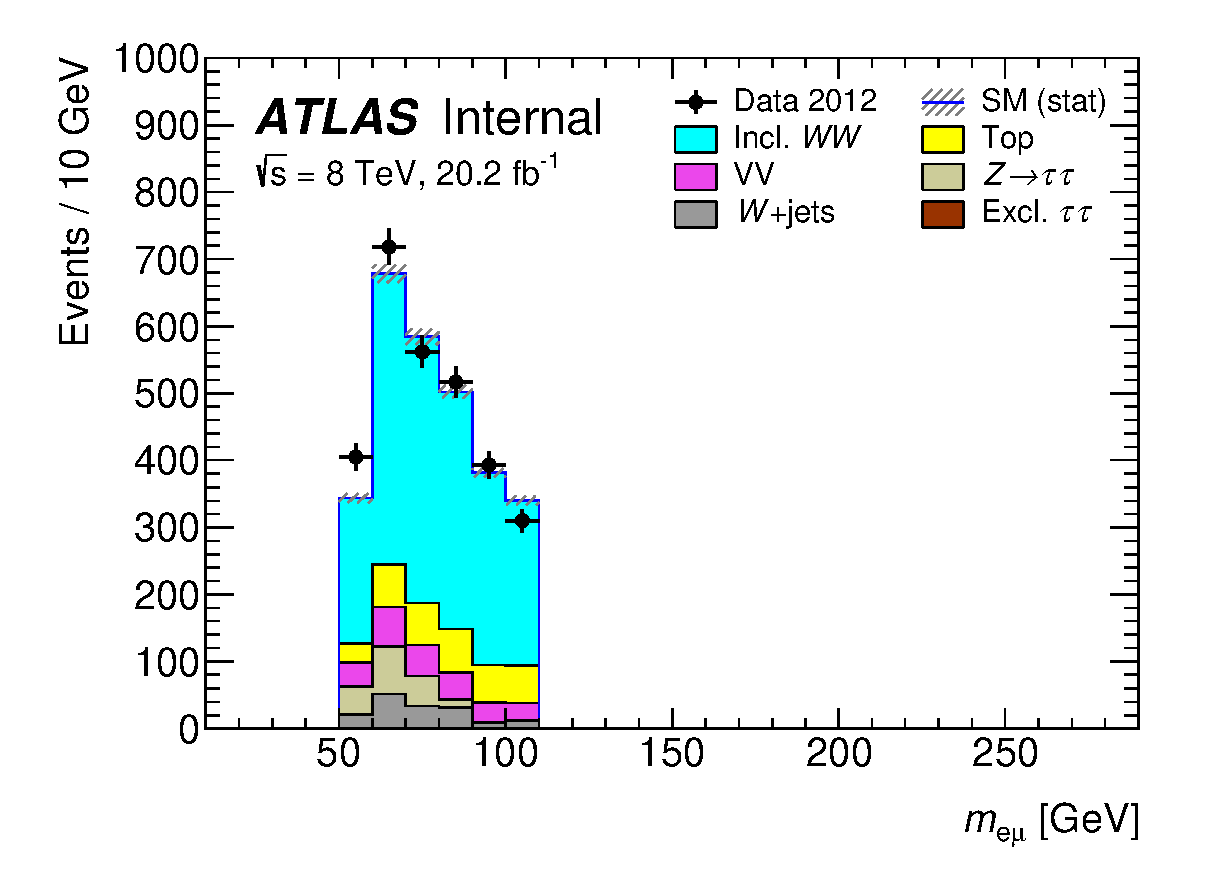
\includegraphics[width=\textwidth]{figures/emme-CutNjets-Mll-lin.eps}
\end{subfigure}
\begin{subfigure}{0.5\textwidth}
   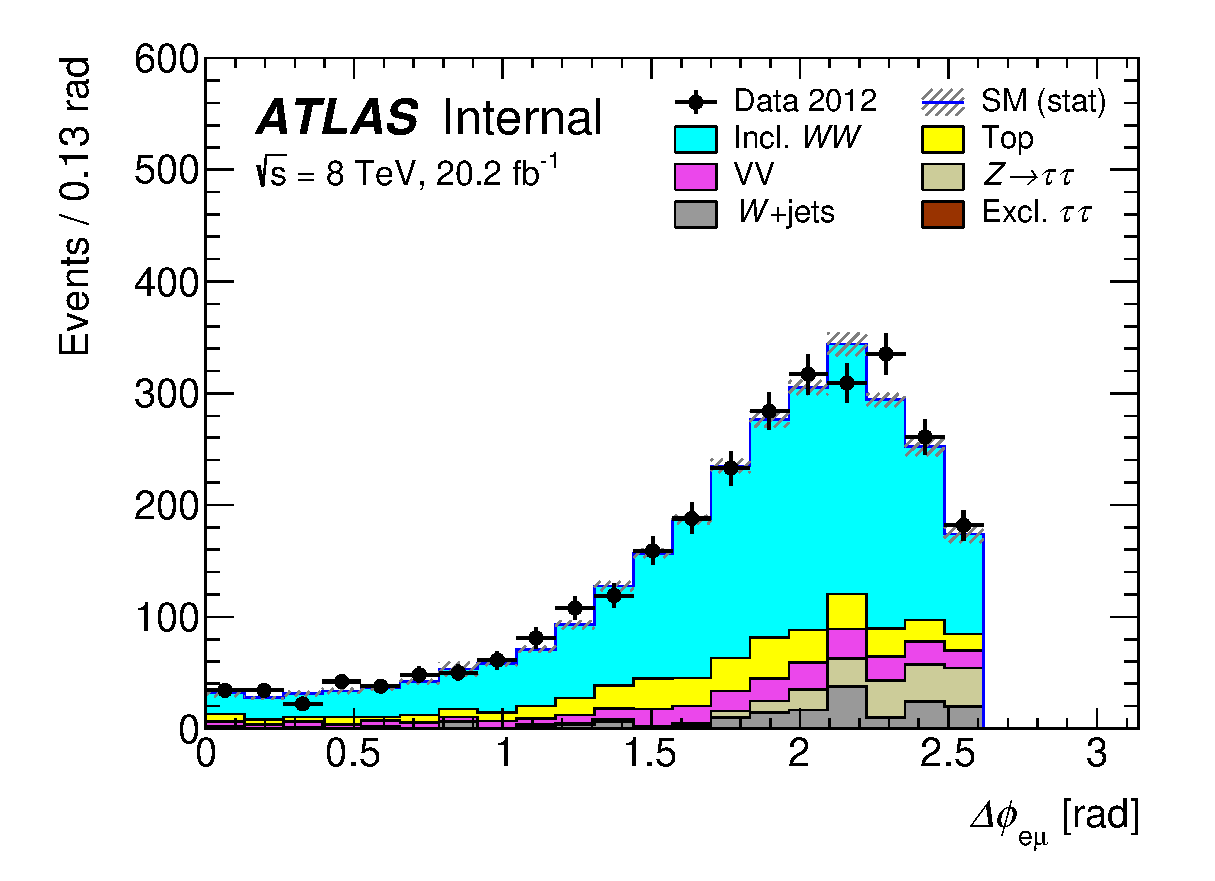
\includegraphics[width=\textwidth]{figures/emme-CutNjets-DPhill-lin.eps}
\end{subfigure} 
\begin{subfigure}{0.5\textwidth}
   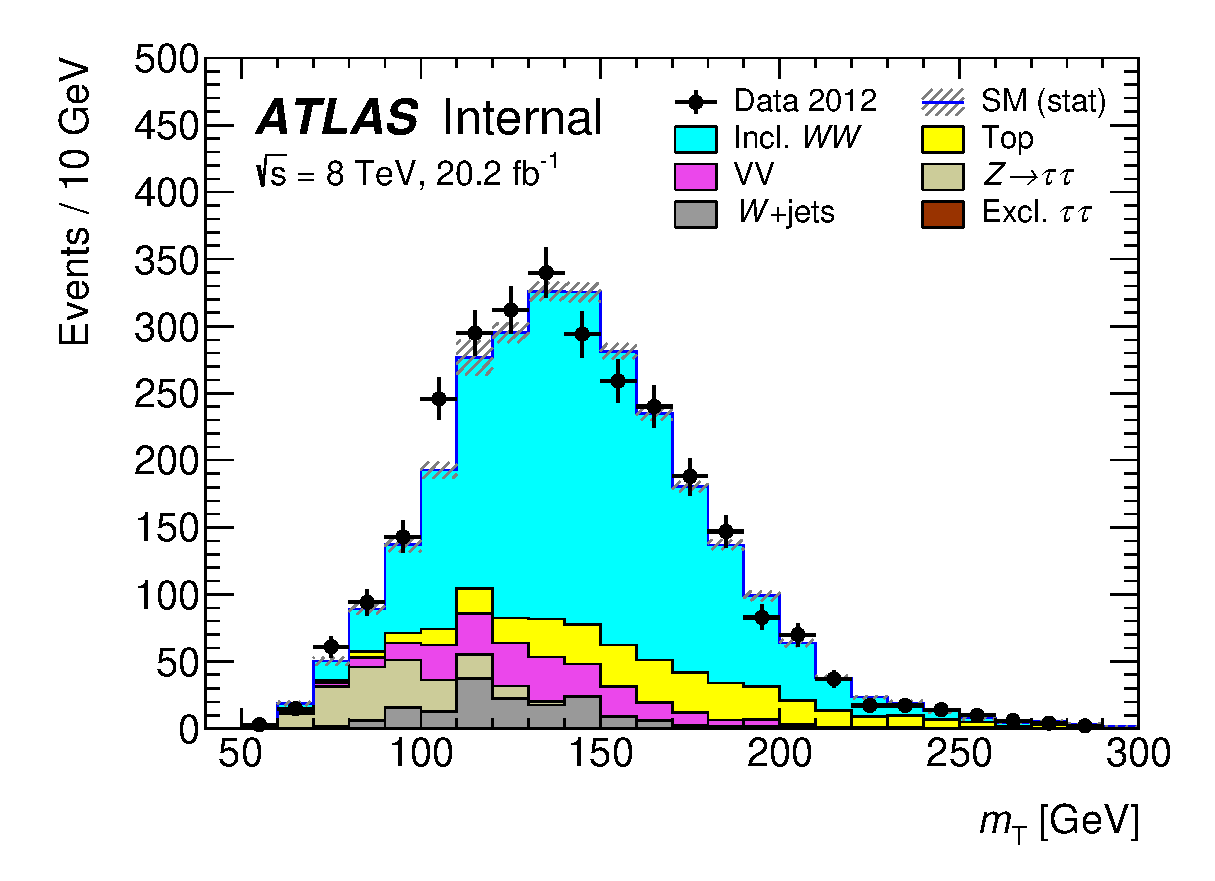
\includegraphics[width=\textwidth]{figures/emme-CutNjets-MT-lin.eps}
\end{subfigure} 
\begin{subfigure}{0.5\textwidth}
   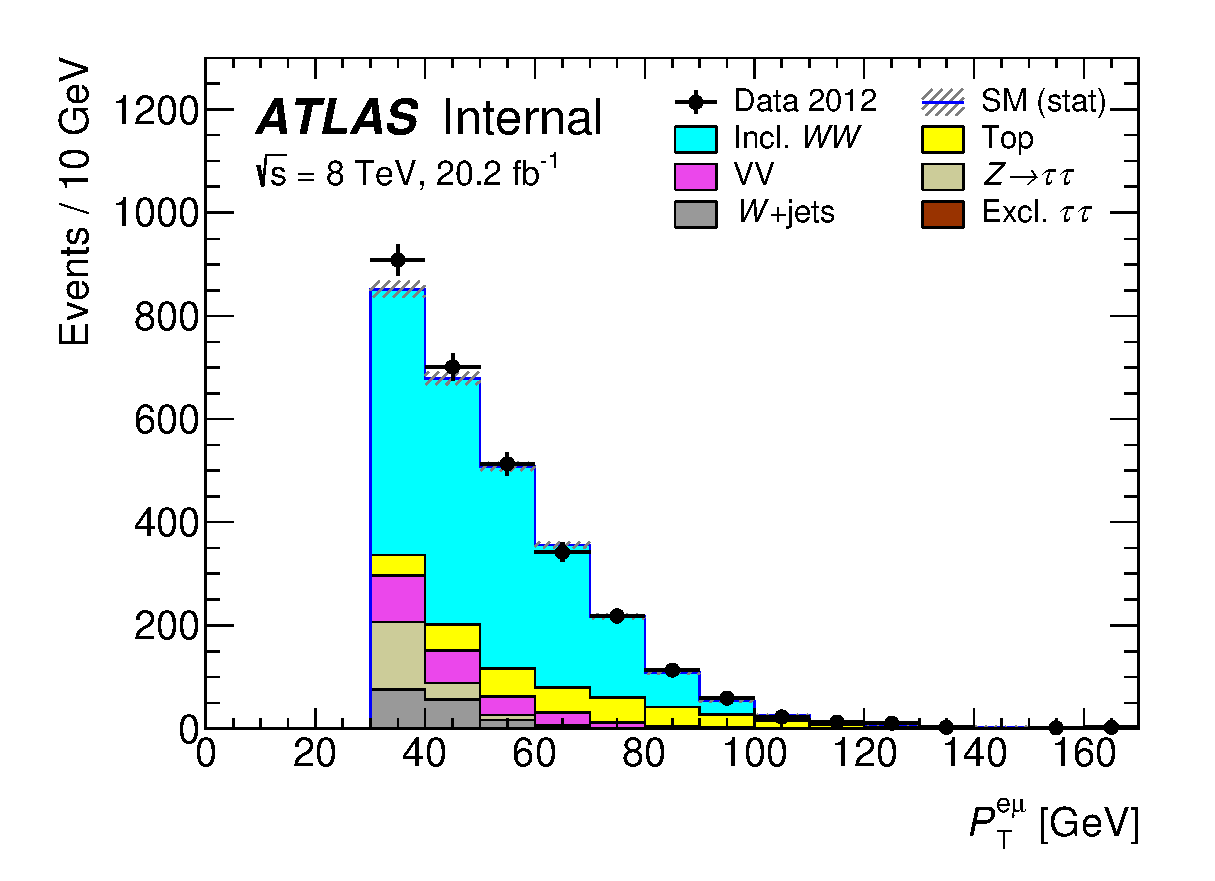
\includegraphics[width=\textwidth]{figures/emme-CutNjets-Ptll-lin.eps}
\end{subfigure} 
\caption{Plots showing \memu, \dFem, \mT\ and \pTemu\ distributions in an inclusive $\WW$-rich region}
\label{fig:incWWplots}
\end{figure}


\subsubsection{Inclusive \WW\ and other backgrounds}
\label{sec:incWW}
\par While the study discussed in the preceding sub-section demonstrates that the inclusive 
\WW\ prediction after correction with the $1.20 \pm 0.05$(stat.) normalization factor was reasonable, 
validation of modelling of inclusive \WW\ after the exclusivity selection was necessary. 
A dedicated control region in data that isolated inclusive \WW\ events to a reasonable 
purity was defined for this purpose. The region definition is listed in Table~\ref{tab:incWWCR}. 

\begin{table}
\centering
\begin{tabular}{|l|c|}
\hline
                                & Selection \\
\hline\hline
& \\
\multirow{3}{*}{Preselection } & Oppositely charged $e\mu$ final states   \\
                                				&  $\pT^{\ell 1} > 25~\GeV$ and $\pT^{\ell 2} > 20~\GeV$ \\
																		    & $\memu > 20~\GeV$     \\
& \\
\hline
& \\
				& $\pTemu > 30~\GeV$\\
                          & Exclusivity selection, allowing 1 to 4 tracks\footnote{\DZ\ allows 0 tracks in 
the exclusivity window.}\\
& \\
\hline
\end{tabular}
\caption{Selection criteria for the region used to study inclusive \WW\ events.}  
\label{tab:incWWCR}
\end{table}

\par The strategy here was to loosen the exclusivity selection slightly by allowing 1 to 4 extra 
tracks in the exclusivity window rather than allowing 0 tracks. While this loose selection allowed 
many inclusive \WW\ events to be selected, rejection of other backgrounds  
was rather unoptimized. These backgrounds are $W$+jets, Drell-Yan and Top. They are referred to here 
as {\it Other Backgrounds}. Exclusive processes such as exclusive \WW\ and exclusive \yytautau, being well 
calibrated by \fgam, were subtracted from the data. This strategy therefore studies the sum of   
inclusive \WW\ and other backgrounds. Expected and observed event yields in this data 
region are listed in Table~\ref{tab:xtrkWWEventYields}, and kinematic distributions are 
shown in Figure~\ref{fig:xtrkWWplots}. 

\begin{table}[!h]
   \centering
   \begin{tabular}{l|c}
     \hline\hline
    Processes & Inclusive $\WW$ \\
    \hline\hline
    Inclusive $\WW$             & 102 $\pm$ 20 \\
    Exclusive $\WW$             & 5.5 $\pm$ 0.4 \\
    Exclusive $\tau^+\tau^-$    & 1.2 $\pm$ 0.2 \\
    Other diboson               & 10.9 $\pm$ 2.2  \\
    Other background            & 27.4 $\pm$ 6.2 \\
    \hline
    Total SM                    & 147 $\pm$ 21  \\
    Data                        & 191             \\
    \hline\hline                                  
   \end{tabular}
  \caption{Event yields in the inclusive $\WW$-rich region.}
  \label{tab:xtrkWWEventYields}
\end{table}

\begin{figure}[!h]
\begin{subfigure}{0.5\textwidth}
   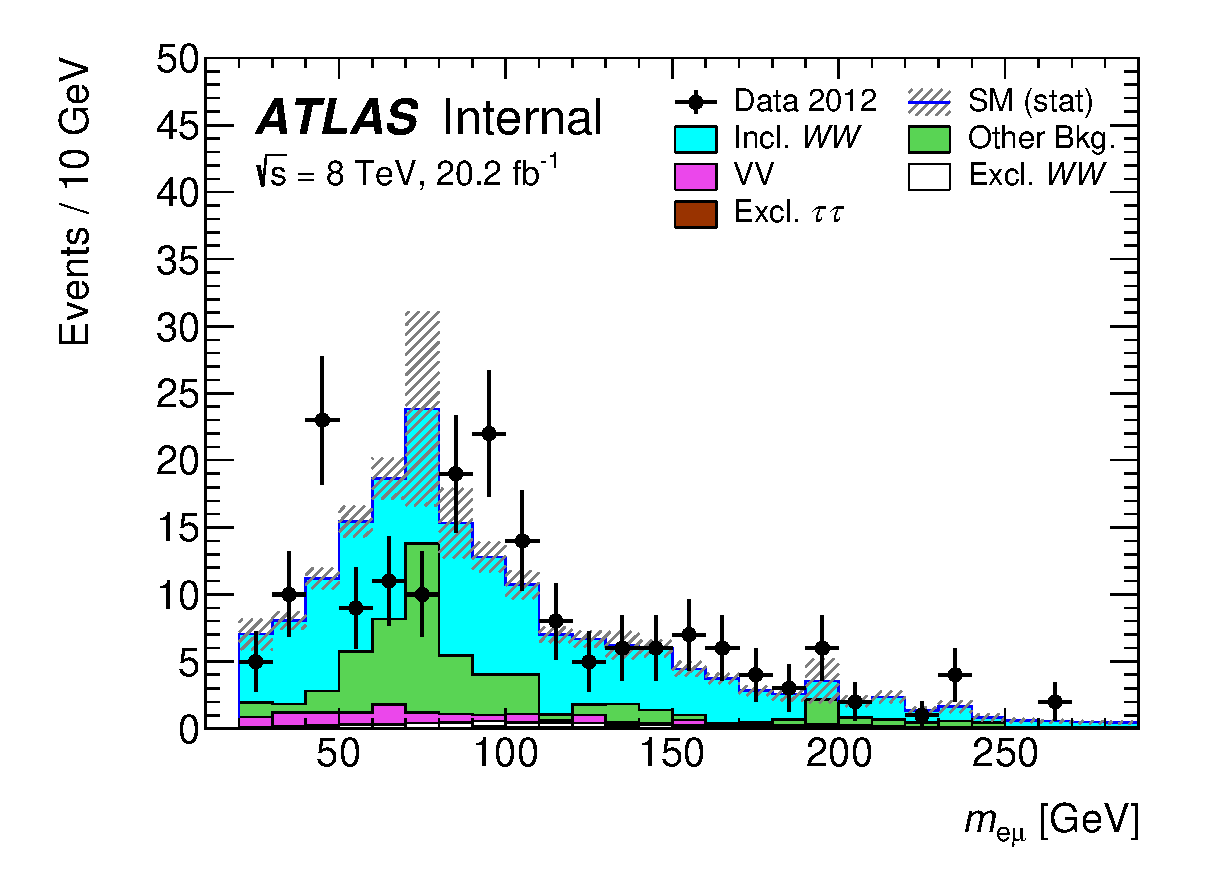
\includegraphics[width=\textwidth]{figures/emme-xtraTracks-Mll-lin.eps}
\end{subfigure}
\begin{subfigure}{0.5\textwidth}
   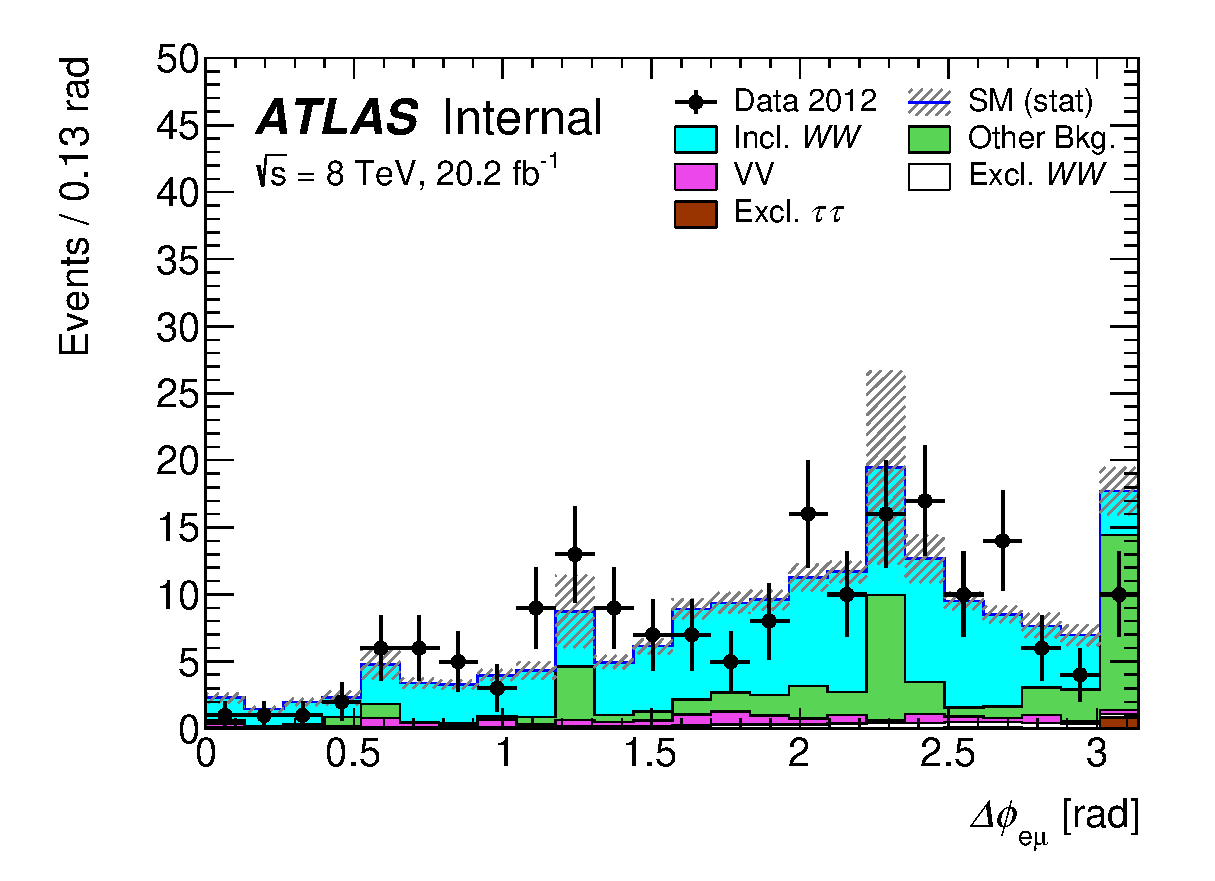
\includegraphics[width=\textwidth]{figures/emme-xtraTracks-DPhill-lin.eps}
\end{subfigure} 
\begin{subfigure}{0.5\textwidth}
   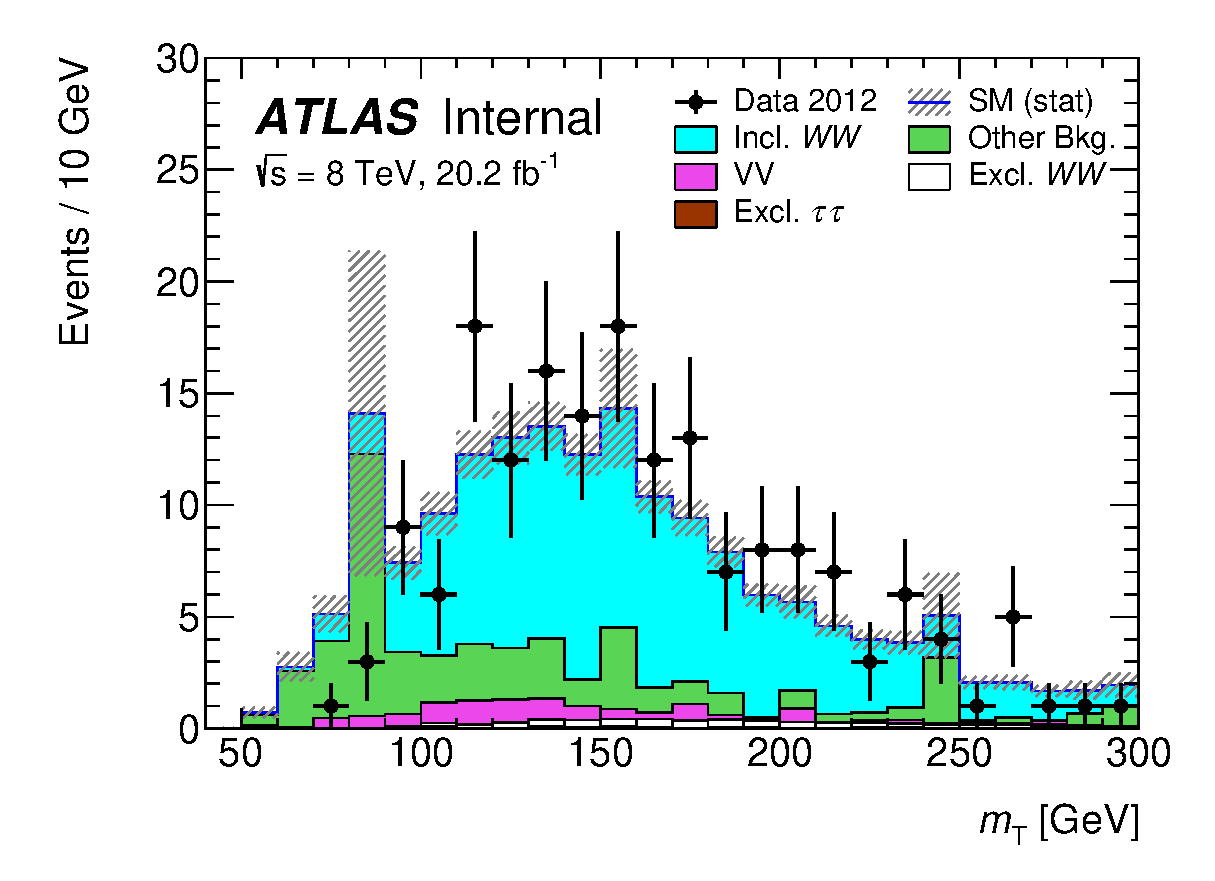
\includegraphics[width=\textwidth]{figures/emme-xtraTracks-MT-lin.eps}
\end{subfigure} 
\begin{subfigure}{0.5\textwidth}
   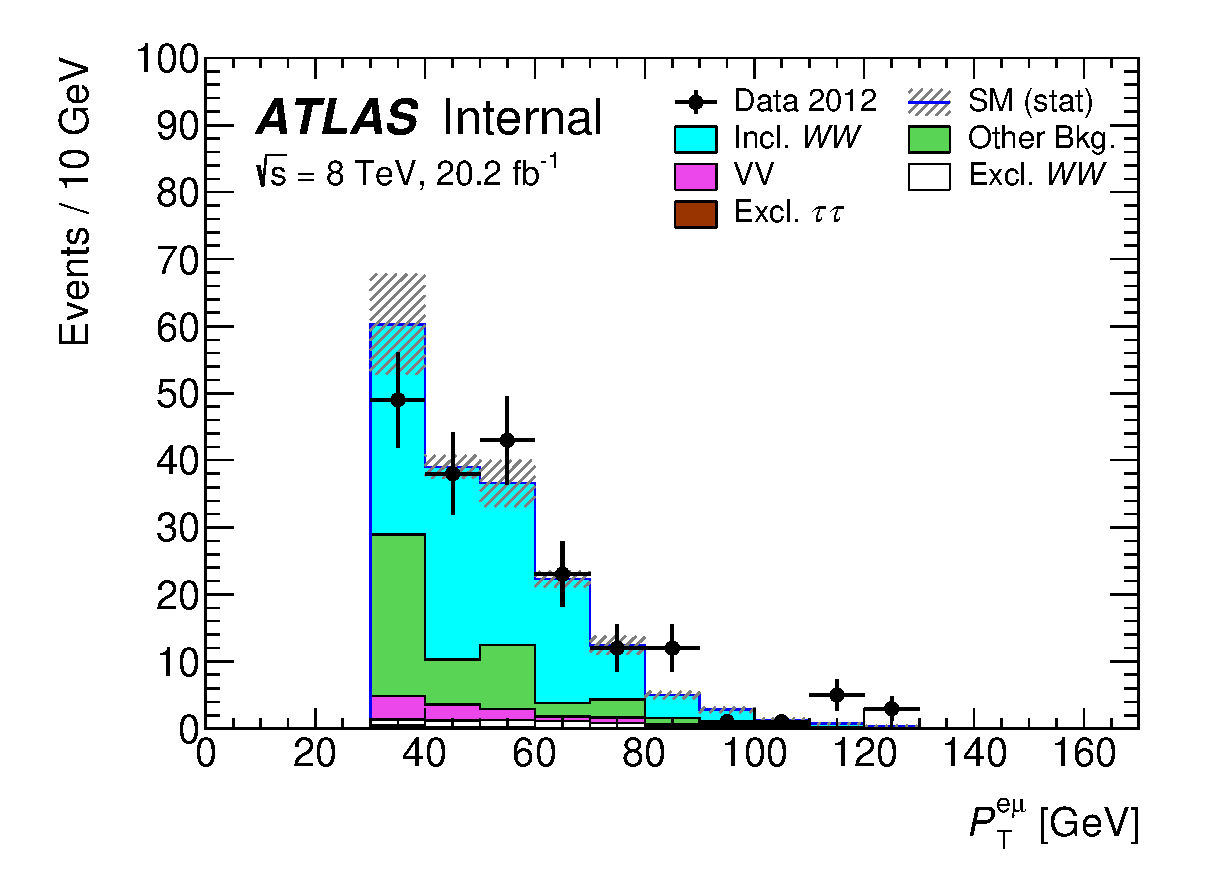
\includegraphics[width=\textwidth]{figures/emme-xtraTracks-Ptll-lin.eps}
\end{subfigure} 
\caption{Plots showing \memu, \dFem, \mT\ and \pTemu\ distributions in the inclusive $\WW$-rich region}
\label{fig:xtrkWWplots}
\end{figure}

\par The true value of the sum of inclusive \WW\ and other backgrounds in this control region     
is bound by two estimates. The upper bound is the observed number of events in data, minus the 
sum of $VV$ and exclusive backgrounds. The lower bound is a special case where there is no 
contribution from the other backgrounds, leading to contribution only from the inclusive \WW, as 
predicted by \PowhegPythiaEight. These two estimates were extrapolated to a region with the same selection criteria but the 
nominal \DZ\ selection.\footnote{In other words, extrapolated from the 1 to 4 track region to the 0 track region}
In this region, the lower bound corresponds to the optimistic case where the other background 
contribution is completely rejected by \DZ, while the upper 
bound corresponds to the case where all observed candidates in the `1 to 4'-track control region are suppressed 
by the same factor as the inclusive $\WW$ process. The average of the two estimates was taken as the 
better estimate to the true value of the sum of inclusive \WW\ and other backgrounds, when the nominal 
\DZ\ selection criterion was applied. Comparing this estimate to the prediction by \PowhegPythiaEight, 
a flat scale factor was extracted to correct for overall exclusivity mis-modelling by Monte Carlo 
simulation. 

\par The extrapolation of upper and lower bounds from the 1 to 4-track region to the nominal \DZ\ region 
was done through 

\begin{equation}
N^{\textrm{Estimated}}_{0} = N^{\textrm{Estimated}}_{1-4} 
                       \times \frac{N_{WW,0}^{\textrm{Predicted}}}{N_{WW,1-4}^{\textrm{Predicted}}}.
\end{equation} 

Here, $N^{\textrm{Estimated}}_{0}$ and $N^{\textrm{Estimated}}_{1-4}$ 
are the estimates for the lower bound or upper bound in the nominal \DZ\ and 1 to 4-track 
region respectively. $N_{WW,0}^{\textrm{Predicted}}$ 
and $N_{WW,1-4}^{\textrm{Predicted}}$ are respectively the number of inclusive $\WW$ events predicted 
by $\PowhegPythiaEight$ for the zero-track and 1 to 4-track regions. 
Extrapolation of the lower bound is trivial: since $N^{\textrm{Estimated}}_{1-4}=N_{WW,1-4}^{\textrm{Predicted}}$ 
the estimate in the nominal \DZ\ region $N^{\textrm{Estimated}}_{0}$ becomes $N_{WW,1-4}^{\textrm{Predicted}}$. 
For upper bound assumes that other backgrounds can be extrapolated using  
$N_{WW,0}^{\textrm{Predicted}}/N_{WW,1-4}^{\textrm{Predicted}}$. The average of 
these two estimates was taken as the overall estimate. Half the difference of the two estimates was taken 
as an additional contribution to the uncertainty in this extrapolation. 

\par This extrapolation yields an estimate of 6.6$\pm$2.5 inclusive \WW\ events in the \DZ\ region. In other 
words, for $\PowhegPythiaEight$ prediction to match this value, a normalization factor of 0.79 was necessary. 
So in the signal region, a 0.79 scale factor was applied to the inclusive \WW\ prediction from Monte Carlo 
simulation. 
 
